\documentclass[12pt]{article} % Base font size of the document.

% Global paragraph formatting
\setlength{\parindent}{20pt} % Adds a consistent indentation for each paragraph
\setlength{\parskip}{0.5em}   % Adds space between paragraphs

% Language setting
% Replace `english' with e.g. `spanish' to change the document language
\usepackage[english]{babel}

% Set page size and margins
% Replace `letterpaper' with`a4paper' for UK/EU standard size
\usepackage[letterpaper,top=3cm,bottom=2cm,left=2cm,right=2cm,marginparwidth=1.75cm]{geometry}

% Useful packages
% \usepackage{times} % font type
% \usepackage{helvet} % font type
% \usepackage{lmodern} % font type
% \usepackage{palatino} % font type
\usepackage{charter} % font type
\usepackage{amsmath}
\usepackage{algorithm}
\usepackage{algpseudocode}
\usepackage{graphicx}
\usepackage{hyperref}
\hypersetup{
    colorlinks=true, % set true if you want colored links
    linktoc=all,     % set to all if both section and subsection linked
    linkcolor=black, % choose some color if you want links to stand out
}
\usepackage{tocloft}
\usepackage{titling}
\usepackage{titlesec}
\usepackage{changepage}
\usepackage[backend=biber, style=numeric, sorting=none]{biblatex}
\addbibresource{Reference.bib} % Specifies the.bib file that stores the document
% \usepackage{indentfirst}

% Customizations
\renewcommand{\cftsecleader}{\cftdotfill{\cftdotsep}}
\renewcommand{\thepage}{\roman{page}} % Roman numerals for title and contents

% Define a custom font size for the title
\newcommand{\titlefont}{\fontsize{28}{36}\selectfont} % You can adjust 35pt font size and 42pt line spacing as needed

% Title and author details
\title{
    {\titlefont\centering James-Stein Estimation and\\Ridge Regression}\\[1ex] % Main title
    \Large MA677 Final Project\\[3ex] % Subtitle
} % Apply the custom font size to the title
\author{Fengyuan (Vincent) Shen\\[3ex]}
\date{\vfill Department of Mathematics and Statistics\\Boston University\\[2ex] May 6, 2024} % Position the department and date at the bottom

% Title page customization
\pretitle{\begin{center}
  
\includegraphics[width=10cm]{images/Boston-University-Logo.png}\\[\bigskipamount] % Include BU logo
  
\includegraphics[width=5cm]{images/MSSP_logo.png}\\[\bigskipamount] % Include MSSP logo
}
\posttitle{\end{center}}


\preauthor{\begin{center}\LARGE}
\postauthor{\end{center}}

\predate{\begin{center}\Large}
\postdate{\end{center}}

% Contents
% To make the title of the contents bold and larger
\renewcommand{\cfttoctitlefont}{\hfill\huge\bfseries} % Change \Large to adjust size
\renewcommand{\cftsecpagefont}{\normalsize} % Section page numbers not in bold

\renewcommand{\cftaftertoctitle}{\hfill\mbox{}\vspace*{0.8cm}}

% Section titles in TOC
\renewcommand{\cftsecfont}{\normalsize\bfseries} % Section titles in bold
\renewcommand{\cftsecpagefont}{\normalsize} % Section page numbers not in bold

% Adjust space between TOC items for sections
\setlength{\cftbeforesecskip}{1.0em}

% Subsection titles in TOC
\renewcommand{\cftsubsecfont}{\normalsize} % Subsection titles not in bold
\renewcommand{\cftsubsecpagefont}{\normalsize} % Subsection page numbers not in bold

% Adjust space between TOC items for subsections
\setlength{\cftbeforesubsecskip}{0.5em} % Adjust this value as needed

% Adjust space between TOC items for subsubsections
\setlength{\cftbeforesubsubsecskip}{0.5em} % Adjust this value as needed

% Chapter title
% Section title formatting
% \titleformat*{\section}{\LARGE\bfseries\centering}
\titleformat{\section} % Command to format the section titles
  [hang] % Shape/style of title
  {\normalfont\huge\bfseries\centering} % Format applied to title: Large, bold, centered
  {} % Label (e.g., "Section")
  {0pt} % Separation between label and title body
  {} % Code preceding the title body

% Subsection title formatting
\titleformat{\subsection}
  {\normalfont\Large\bfseries} % Change to \large for larger size
  {\thesubsection} % Label is subsection number
  {1em} % Space between number and title
  {} % Optional code

% Subsubsection title formatting
\titleformat{\subsubsection}
  {\normalfont\large\bfseries} % Change to \normalsize or larger if needed
  {\thesubsubsection} % Label is subsubsection number
  {1em} % Space between number and title
  {} % Optional code


\begin{document}

\begin{titlingpage}
\maketitle
\thispagestyle{empty} % No page number on the title page
\end{titlingpage}

\newpage
% \begin{center}
%     \huge \textbf{Abstract}
% \end{center}

% Add the abstract to the Table of Contents
\addcontentsline{toc}{section}{Abstract}

\section*{Abstract}

\begin{quote}
    This paper examines the advancements in statistical estimation through the integration of shrinkage techniques, specifically the James-Stein Estimator and Ridge Regression, within an empirical Bayes framework. These methods demonstrate significant improvements in estimation accuracy and reliability, particularly in scenarios involving small sample sizes or high-dimensional data. The exploration begins with a deep dive into the mathematical foundations of these estimators, providing proofs of their superiority over traditional methods and linking their theoretical underpinnings. Practical computational methods are then applied to illustrate their effectiveness through simulations and comparative analyses. Finally, the implications of these techniques are discussed, emphasizing their role in enhancing the dependability of statistical predictions and addressing challenges such as overfitting and multicollinearity. This study highlights the practical and conceptual benefits of shrinkage methods in statistical practice, showcasing their potential to revolutionize traditional estimation approaches.\\
    \\
    \textbf{Keywords:} \textit{James-Stein Estimator, Empirical Bayes, Ridge Regression}
\end{quote}
\thispagestyle{empty} % No page number on abstract

\newpage
\tableofcontents

\newpage
\setcounter{page}{1} % Start counting pages
\renewcommand{\thepage}{\arabic{page}} % Arabic numerals for the rest of the document

% Include the chapters
% % \begin{center}
%     \huge \textbf{Abstract}
% \end{center}

% Add the abstract to the Table of Contents
\addcontentsline{toc}{section}{Abstract}

\section*{Abstract}

\begin{quote}
    This paper examines the advancements in statistical estimation through the integration of shrinkage techniques, specifically the James-Stein Estimator and Ridge Regression, within an empirical Bayes framework. These methods demonstrate significant improvements in estimation accuracy and reliability, particularly in scenarios involving small sample sizes or high-dimensional data. The exploration begins with a deep dive into the mathematical foundations of these estimators, providing proofs of their superiority over traditional methods and linking their theoretical underpinnings. Practical computational methods are then applied to illustrate their effectiveness through simulations and comparative analyses. Finally, the implications of these techniques are discussed, emphasizing their role in enhancing the dependability of statistical predictions and addressing challenges such as overfitting and multicollinearity. This study highlights the practical and conceptual benefits of shrinkage methods in statistical practice, showcasing their potential to revolutionize traditional estimation approaches.\\
    \\
    \textbf{Keywords:} \textit{James-Stein Estimator, Empirical Bayes, Ridge Regression}
\end{quote}
\include{chapter1}
\include{chapter2}
\include{chapter3}
\section{Computational Methods}

This section focuses on practical computational approaches to implementing the James-Stein Estimator and Ridge Regression. Through simulations and comparisons, we demonstrate the effectiveness of these methods in statistical estimation.

\subsection{Implementing James-Stein Estimator}

The James-Stein Estimator is implemented to demonstrate its shrinkage effect on simulated data. This estimator is particularly notable for its ability to reduce estimation errors by shrinking estimates towards their overall mean.

\subsubsection{Algorithm for James-Stein Estimator}
\begin{algorithm}
\caption{James-Stein Estimator}
\begin{algorithmic}[1]
\Procedure{JamesSteinEstimator}{$z$, $sigma\_squared$}
    \State $n \gets \text{length}(z)$
    \State $z\_bar \gets \text{mean}(z)$
    \State $s\_squared \gets \text{sum}((z - z\_bar)^2) / n$
    \State $shrinkage\_factor \gets 1 - ((n-3) * sigma\_squared / s\_squared)$
    \State $shrinkage\_factor \gets \text{max}(0, shrinkage\_factor)$
    \For{$i \gets 1$ to $n$}
        \State $z[i] \gets z\_bar + shrinkage\_factor * (z[i] - z\_bar)$
    \EndFor
    \State \textbf{return} $z$
\EndProcedure
\end{algorithmic}
\end{algorithm}

\subsubsection{Simulation Results}

Data are generated from a normal distribution with a mean of 5 and a standard deviation of 1. The James-Stein Estimator is then applied to these data, demonstrating significant shrinkage of estimates towards the mean. The impact of this shrinkage is clearly illustrated in a scatter plot that compares the original data with the James-Stein estimation.

\begin{figure}[H]
    \centering
    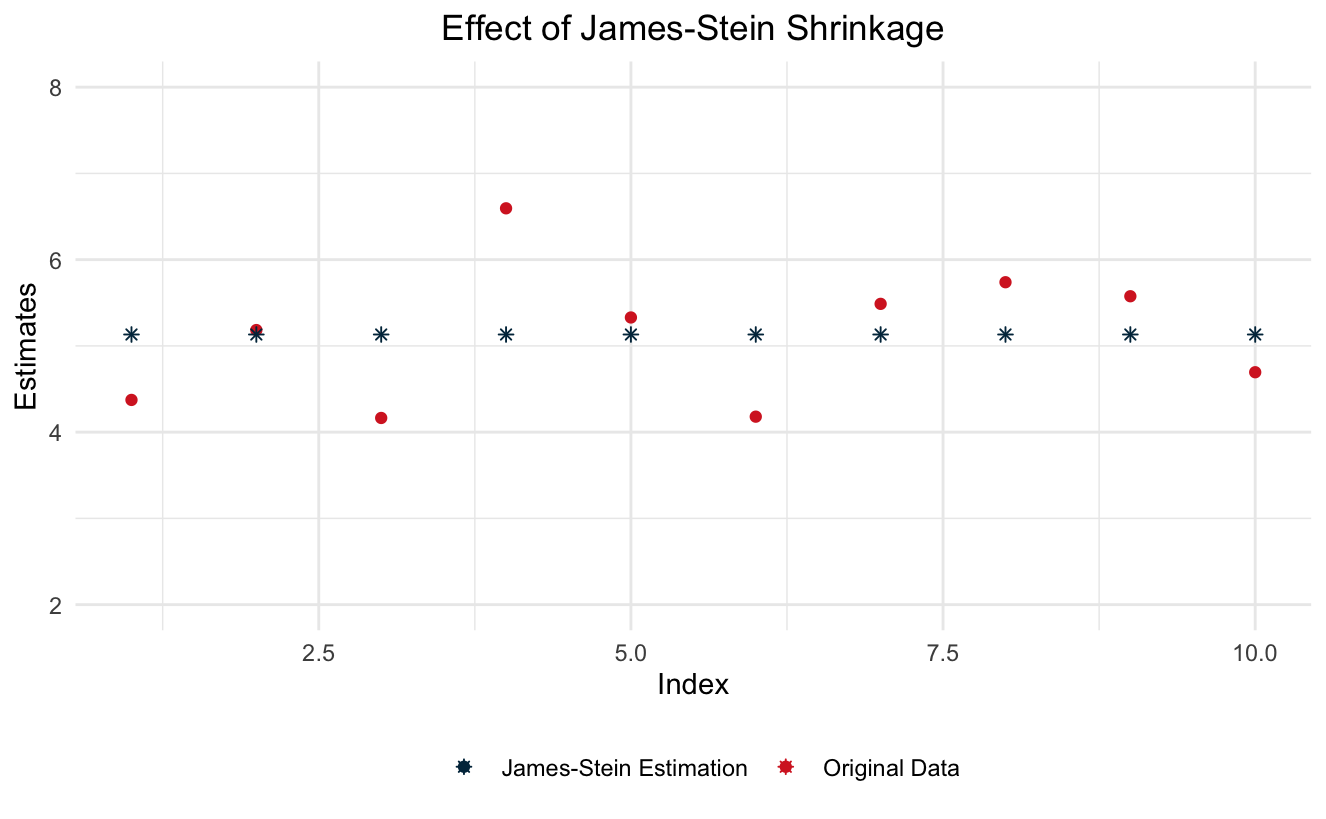
\includegraphics[width=1\textwidth]{images/Effect of James-Stein Shrinkage.png}
    \caption{Effect of James-Stein shrinkage on simulated data.}
    \label{fig:jse_shrinkage}
\end{figure}

\subsection{Simulation of Estimator Effectiveness}

We compare the James-Stein Estimator with the Maximum Likelihood Estimator across different sample sizes to illustrate the reduction in squared errors.

\newpage

\subsubsection{Algorithm for Comparing Estimator Effectiveness}
\begin{algorithm}
\caption{Compare Estimators}
\begin{algorithmic}[1]
\Procedure{CompareEstimators}{$num\_sim$, $sample\_sizes$, $mu$, $sigma$}
    \For{$n$ in $sample\_sizes$}
        \State $mle\_errors \gets$ vector of size $num\_sim$
        \State $jse\_errors \gets$ vector of size $num\_sim$
        \For{$i \gets 1$ to $num\_sim$}
            \State $z \gets \text{generate normal data}(n, mu, sigma)$
            \State $mle \gets \text{mean}(z)$
            \State $s\_squared \gets \text{sum}((z - mle)^2) / n$
            \State $shrinkage\_factor \gets 1 - ((n-3) * sigma^2 / s\_squared)$
            \State $shrinkage\_factor \gets \text{max}(0, shrinkage\_factor)$
            \State $jse \gets mle + shrinkage\_factor * (z - mle)$
            \State $mle\_errors[i] \gets \text{sum}((mle - mu)^2)$
            \State $jse\_errors[i] \gets \text{sum}((jse - mu)^2)$
        \EndFor
        \State Store $mle\_errors$ and $jse\_errors$ in data frame
    \EndFor
    \State \textbf{return} data frame
\EndProcedure
\end{algorithmic}
\end{algorithm}

\subsubsection{Visualizing Comparison Results}

The log-squared errors of both estimators are plotted to show the James-Stein Estimator's efficiency, especially in smaller samples.

Generally, the James-Stein Estimator demonstrates lower median log squared errors compared to the MLE across all sample sizes, particularly as the sample size increases. This demonstrates the effectiveness of the James-Stein shrinkage, especially in reducing variance and improving estimation accuracy over the traditional MLE approach.

\begin{figure}[H]
    \centering
    \includegraphics[width=1\textwidth]{images/Comparison of MLE and James–Stein Estimator Errors.png}
    \caption{Log-squared error comparison of MLE and JSE across different sample sizes.}
    \label{fig:estimators_comparison}
\end{figure}

\subsection{Exploring Ridge Regression}

Ridge Regression is investigated as an auxiliary method that also demonstrates shrinkage, similar to the James-Stein approach, but within the framework of regression analysis. Data and coefficients are generated and Ridge Regression is implemented using the glmnet package in R.

The plot of coefficient shrinkage, as the regularization parameter increases, showcases Ridge Regression's capacity to effectively manage overfitting and multicollinearity, highlighting its utility in high-dimensional statistical modeling.

\begin{figure}[H]
    \centering
    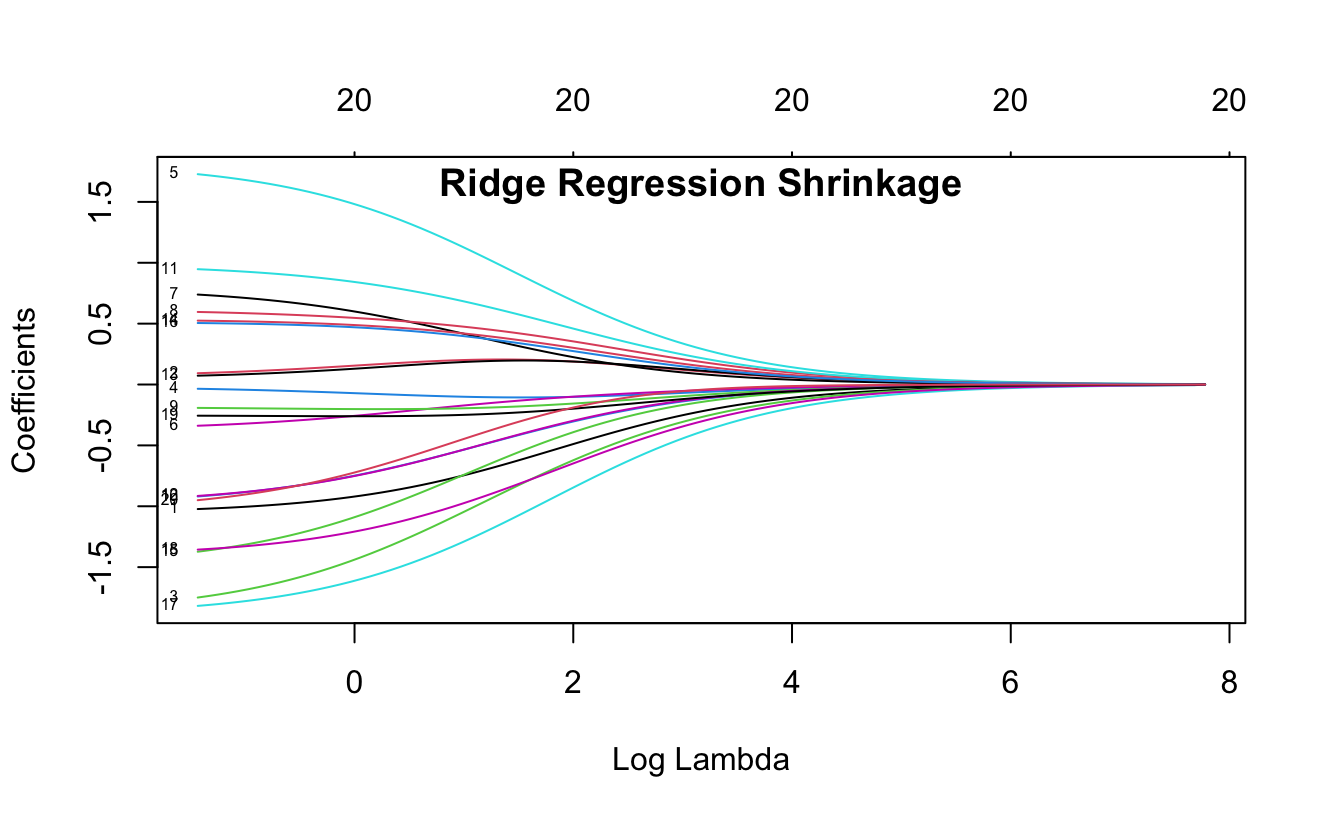
\includegraphics[width=1\textwidth]{images/Ridge Regression Shrinkage.png}
    \caption{Coefficient shrinkage in Ridge Regression as a function of the regularization parameter.}
    \label{fig:ridge_shrinkage}
\end{figure}

\subsection{Conclusion}

This section has showcased the practical utility and advantages of the James-Stein Estimator and Ridge Regression through detailed computational demonstrations. Both methods are united by their use of shrinkage to enhance the accuracy and dependability of statistical estimates.
\section{Conclusions}

This study has explored the significant impact of the James-Stein Estimator and Ridge Regression on statistical practice, emphasizing their conceptual and practical benefits in improving estimation accuracy and reliability. These methods exemplify the power of shrinkage techniques in addressing challenges in statistical estimation, particularly in scenarios of high dimensionality or small sample sizes.

\subsection{Implications for Statistical Practice}

\begin{itemize}
    \item \textbf{James-Stein Estimator}: With its robust performance improvement over traditional Maximum Likelihood Estimation, especially in the context of small sample sizes, James-Stein Estimator demonstrates a critical advancement in statistical estimation theory. It effectively reduces estimation error by leveraging the strength of shrinkage towards the mean, which is particularly beneficial in empirical Bayesian contexts. This approach not only enhances the reliability of estimates but also provides a substantial reduction in the risk of overfitting, making it an invaluable tool in statistical analysis.
    \item \textbf{Ridge Regression}: It complements the James-Stein Estimator by applying similar principles of shrinkage within a regression framework. This technique addresses the limitations of Ordinary Least Squares estimation in the presence of multicollinearity or when the number of predictors exceeds the number of observations. By introducing a penalty term that constrains the size of the coefficients, Ridge Regression ensures more stable and interpretable models, which is crucial for complex data analyses involving numerous predictors.
\end{itemize}

\subsection{Synthesis of Key Findings}

The integration of computational methods to illustrate the efficacy of these estimators underscores their practical significance in real-world applications. The James-Stein Estimator's ability to shrink estimates toward the overall mean offers a pragmatic solution for enhancing the accuracy of predictions derived from small datasets or datasets with high variance in observations. Similarly, Ridge Regression's capability to manage the complexity of models by penalizing the magnitude of coefficients helps in mitigating issues arising from overfitting and multicollinearity, promoting more reliable predictive modeling.


% Add a reference section
\newpage
\printbibliography[heading=bibintoc, title={References}]

% Mark the beginning of the appendix
\newpage
\appendix
\section{Appendix}

\subsection{R Code for Implementation of the James-Stein Estimator}

\begin{verbatim}
# Function to apply James-Stein Estimator
james_stein_estimator <- function(z, sigma_squared) {
  n <- length(z)
  z_bar <- mean(z)
  s_squared <- sum((z - z_bar)^2) / n
  shrinkage_factor <- 1 - ((n-3) * sigma_squared / s_squared)
  shrinkage_factor <- max(0, shrinkage_factor)  # Ensure non-negative shrinkage
  return(z_bar + shrinkage_factor * (z - z_bar))
}

# Simulate data
set.seed(1)
z <- rnorm(10, mean = 5, sd = 1)
sigma_squared <- 1

# Apply the JSE
jse_results <- james_stein_estimator(z, sigma_squared)
print(jse_results)

data <- data.frame(Index = 1:length(z),
                   Original = z,
                   JamesStein = jse_results)

ggplot(data) +
  geom_point(aes(x = Index, y = Original, color = "Original Data"), pch = 19) +
  geom_point(aes(x = Index, y = JamesStein, color = "James-Stein Estimation"), pch = 8) +
  scale_color_manual(values = c("Original Data" = "#d62828", 
                                "James-Stein Estimation" = "#003049")) +
  labs(x = "Index", y = "Estimates", title = "Effect of James-Stein Shrinkage") +
  theme_minimal() +
  theme(
    plot.title = element_text(hjust = 0.5),
    legend.title = element_blank(),
    legend.position = 'bottom'
    ) +
  ylim(2, 8)
\end{verbatim}

\subsection{R Code for Simulation of Estimator Effectiveness}

\begin{verbatim}
# Perform simulations and calculate MLE and JSE
simulate_estimators <- function(n, mu = 5, sigma = 1, num_sim = 1000) {
  mle_errors <- numeric(num_sim)
  jse_errors <- numeric(num_sim)
  
  for (i in 1:num_sim) {
    z <- rnorm(n, mean = mu, sd = sigma)
    mle <- mean(z)
    s_squared <- sum((z - mle)^2) / n
    shrinkage_factor <- 1 - ((n-3) * sigma^2 / s_squared)
    shrinkage_factor <- max(0, shrinkage_factor)
    jse <- mle + shrinkage_factor * (z - mle)
    
    mle_errors[i] <- sum((mle - mu)^2)
    jse_errors[i] <- sum((jse - mu)^2)
  }
  
  data.frame(
    Error = c(jse_errors, mle_errors),
    Estimator = rep(c("err_MLE", "err_JSE"), each = num_sim),
    N = rep(n, 2 * num_sim)
  )
}

# Parameters
sample_sizes <- c(3, 5, 10, 20)
num_simulations <- 1000

# Run simulations for multiple sample sizes
results <- do.call(rbind, lapply(sample_sizes, function(n) {
  simulate_estimators(n = n, num_sim = num_simulations)
}))
results$Estimator <- factor(results$Estimator, levels = c("err_MLE", "err_JSE"))

# Plot
ggplot(results, aes(x = Estimator, y = log(Error + 1), fill = Estimator)) +
  geom_boxplot() +
  facet_wrap(~ N, scales = "free") +
  labs(title = "Comparison of MLE and James–Stein Estimator Errors",
       x = "Estimator Type",
       y = "Log Squared Error") +
  theme_minimal() +
  theme(plot.title = element_text(hjust = 0.5)) +
  scale_fill_manual(values = c("err_MLE" = "#d62828", "err_JSE" = "#778da9"))
\end{verbatim}

\subsection{R Code for Comparing with Ridge Regression}

\begin{verbatim}
# Simulate data
set.seed(1)
x <- matrix(rnorm(100*20), 100, 20)  # 100 observations, 20 predictors
beta <- runif(20, -2, 2)  # True coefficients
y <- x %*% beta + rnorm(100)  # Response variable

# Ridge regression using glmnet
fit <- glmnet(x, y, alpha = 0)

# Plot coefficient shrinkage
plot(fit, xvar = "lambda", label = TRUE)
title(main = "Ridge Regression Shrinkage", line = -1)
\end{verbatim}

\end{document}